\documentclass[12pt]{extreport}
\usepackage[T2A]{fontenc}
\usepackage[utf8]{inputenc}        % Кодировка входного документа;
                                    % при необходимости, вместо cp1251
                                    % можно указать cp866 (Alt-кодировка
                                    % DOS) или koi8-r.

\usepackage[english,russian]{babel} % Включение русификации, русских и
                                    % английских стилей и переносов
%%\usepackage{a4}
%%\usepackage{moreverb}
\usepackage{amsmath,amsfonts,amsthm,amssymb,amsbsy,amstext,amscd,amsxtra,multicol}
\usepackage{indentfirst}
\usepackage{verbatim}
\usepackage{tikz} %Рисование автоматов
\usetikzlibrary{automata,positioning}
\usepackage{multicol} %Несколько колонок
\usepackage{graphicx}
\usepackage[colorlinks,urlcolor=blue]{hyperref}
\usepackage[stable]{footmisc}

\usepackage[linesnumbered]{algorithm2e}   
\usepackage{MnSymbol,wasysym}

\usepackage{graphicx}
\usepackage{listings}
\graphicspath{ {.} }

%% \voffset-5mm
%% \def\baselinestretch{1.44}
\renewcommand{\theequation}{\arabic{equation}}
\def\hm#1{#1\nobreak\discretionary{}{\hbox{$#1$}}{}}
\newtheorem{Lemma}{Лемма}
\theoremstyle{definiton}
\newtheorem{Remark}{Замечание}
%%\newtheorem{Def}{Определение}
\newtheorem{Claim}{Утверждение}
\newtheorem{Cor}{Следствие}
\newtheorem{Theorem}{Теорема}
\theoremstyle{definition}
\newtheorem{Example}{Пример}
\newtheorem*{known}{Теорема}
\def\proofname{Доказательство}
\theoremstyle{definition}
\newtheorem{Def}{Определение}



\DeclareMathOperator{\Cov}{Cov}
\DeclareMathOperator{\Var}{Var}
\DeclareMathOperator{\Corr}{Corr}
\DeclareMathOperator{\E}{\mathop{E}}
\DeclareMathOperator{\Med}{Med}
\DeclareMathOperator{\Mod}{Mod}
\DeclareMathOperator*{\plim}{plim}

%% \newenvironment{Example} % имя окружения
%% {\par\noindent{\bf Пример.}} % команды для \begin
%% {\hfill$\scriptstyle\qed$} % команды для \end


% одеваем шапки на частые штуки
\def \hb{\hat{\beta}}
\def \hs{\hat{s}}
\def \hy{\hat{y}}
\def \hY{\hat{Y}}
\def \he{\hat{\varepsilon}}
\def \hVar{\widehat{\Var}}
\def \hCorr{\widehat{\Corr}}
\def \hCov{\widehat{\Cov}}

% Греческие буквы
\def \a{\alpha}
\def \b{\beta}
\def \t{\tau}
\def \dt{\delta}
\def \e{\varepsilon}
\def \ga{\gamma}
\def \kp{\varkappa}
\def \la{\lambda}
\def \sg{\sigma}
\def \tt{\theta}
\def \Dt{\Delta}
\def \La{\Lambda}
\def \Sg{\Sigma}
\def \Tt{\Theta}
\def \Om{\Omega}
\def \om{\omega}

% Готика
\def \mA{\mathcal{A}}
\def \mB{\mathcal{B}}
\def \mC{\mathcal{C}}
\def \mE{\mathcal{E}}
\def \mF{\mathcal{F}}
\def \mH{\mathcal{H}}
\def \mL{\mathcal{L}}
\def \mN{\mathcal{N}}
\def \mU{\mathcal{U}}
\def \mV{\mathcal{V}}
\def \mW{\mathcal{W}}

% Жирные буквы
\def \mbb{\mathbb}
\def \RR{\mbb R}
\def \NN{\mbb N}
\def \ZZ{\mbb Z}
\def \PP{\mbb{P}}
\def \QQ{\mbb Q}



%\date{22 июня 2011 г.}
\let\leq\leqslant
\let\geq\geqslant
\def\MT{\mathrm{MT}}
%Обозначения ``ажуром''
\def\BB{\mathbb B}
\def\CC{\mathbb C}
\def\RR{\mathbb R}
\def\SS{\mathbb S}
\def\ZZ{\mathbb Z}
\def\NN{\mathbb N}
\def\FF{\mathbb F}
%греческие буквы
\let\epsilon\varepsilon
\let\es\varnothing
\let\eps\varepsilon
\let\al\alpha
\let\sg\sigma
\let\ga\gamma
\let\ph\varphi
\let\om\omega
\let\ld\lambda
\let\Ld\Lambda
\let\vk\varkappa
\let\Om\Omega
\def\abstractname{}

\def\R{{\cal R}}
\def\A{{\cal A}}
\def\B{{\cal B}}
\def\C{{\cal C}}
\def\D{{\cal D}}

%классы сложности
\def\REG{{\mathsf{REG}}}
\def\CFL{{\mathsf{CFL}}}


%%%%%%%%%%%%%%%%%%%%%%%%%%%%%%% Problems macros  %%%%%%%%%%%%%%%%%%%%%%%%%%%%%%%


%%%%%%%%%%%%%%%%%%%%%%%% Enumerations %%%%%%%%%%%%%%%%%%%%%%%%

\newcommand{\Rnum}[1]{\expandafter{\romannumeral #1\relax}}
\newcommand{\RNum}[1]{\uppercase\expandafter{\romannumeral #1\relax}}

%%%%%%%%%%%%%%%%%%%%% EOF Enumerations %%%%%%%%%%%%%%%%%%%%%

\usepackage{xparse}
\usepackage{ifthen}
\usepackage{bm} %%% bf in math mode
\usepackage{color}
%\usepackage[usenames,dvipsnames]{xcolor}

\definecolor{Gray555}{HTML}{555555}
\definecolor{Gray444}{HTML}{444444}
\definecolor{Gray333}{HTML}{333333}


\newcounter{problem}
\newcounter{uproblem}
\newcounter{subproblem}
\newcounter{prvar}

\def\beforPRskip{
	\bigskip
	%\vspace*{2ex}
}

\def\PRSUBskip{
	\medskip
}


\def\pr{\beforPRskip\noindent\stepcounter{problem}{\bf \theproblem .\;}\setcounter{subproblem}{0}}
\def\pru{\beforPRskip\noindent\stepcounter{problem}{\bf $\mathbf{\theproblem}^\circ$\!\!.\;}\setcounter{subproblem}{0}}
\def\prstar{\beforPRskip\noindent\stepcounter{problem}{\bf $\mathbf{\theproblem}^*$\negthickspace.}\setcounter{subproblem}{0}\;}
\def\prpfrom[#1]{\beforPRskip\noindent\stepcounter{problem}{\bf Задача \theproblem~(№#1 из задания).  }\setcounter{subproblem}{0} }
\def\prp{\beforPRskip\noindent\stepcounter{problem}{\bf Задача \theproblem .  }\setcounter{subproblem}{0} }

\def\prpvar{\beforPRskip\noindent\stepcounter{problem}\setcounter{prvar}{1}{\bf Задача \theproblem \;$\langle${\rm\Rnum{\theprvar}}$\rangle$.}\setcounter{subproblem}{0}\;}
\def\prpv{\beforPRskip\noindent\stepcounter{prvar}{\bf Задача \theproblem \,$\bm\langle$\bracketspace{{\rm\Rnum{\theprvar}}}$\bm\rangle$.  }\setcounter{subproblem}{0} }
\def\prv{\beforPRskip\noindent\stepcounter{prvar}{\bf \theproblem\,$\bm\langle$\bracketspace{{\rm\Rnum{\theprvar}}}$\bm\rangle$}.\setcounter{subproblem}{0} }

\def\prpstar{\beforPRskip\noindent\stepcounter{problem}{\bf Задача $\bf\theproblem^*$\negthickspace.  }\setcounter{subproblem}{0} }
\def\prdag{\beforPRskip\noindent\stepcounter{problem}{\bf Задача $\theproblem^{^\dagger}$\negthickspace\,.  }\setcounter{subproblem}{0} }
\def\upr{\beforPRskip\noindent\stepcounter{uproblem}{\bf Упражнение \theuproblem.}\setcounter{subproblem}{0}\;}
%\def\prp{\vspace{5pt}\stepcounter{problem}{\bf Задача \theproblem .  } }
%\def\prs{\vspace{5pt}\stepcounter{problem}{\bf \theproblem .*   }
\def\prsub{\PRSUBskip\noindent\stepcounter{subproblem}{\sf \thesubproblem.}\;}
\def\prsubr{\PRSUBskip\noindent\stepcounter{subproblem}{\bf \asbuk{subproblem})}\;}
\def\prsubstar{\PRSUBskip\noindent\stepcounter{subproblem}{\rm $\thesubproblem^*$\negthickspace.}\;}
\def\prsubrstar{\PRSUBskip\noindent\stepcounter{subproblem}{$\text{\bf \asbuk{subproblem}}^*\mathbf{)}$}\;}

\newcommand{\bracketspace}[1]{\phantom{(}\!\!{#1}\!\!\phantom{)}}

\DeclareDocumentCommand{\Prpvar}{ O{null} O{} }{
	\beforPRskip\noindent\stepcounter{problem}\setcounter{prvar}{1}{\bf Задача \theproblem
% 	\ifthenelse{\equal{#1}{null}}{  }{ {\sf $\bm\langle$\bracketspace{#1}$\bm\rangle$}}
%	~\!\!(\bracketspace{{\rm\Rnum{\theprvar}}}).  }\setcounter{subproblem}{0}
%	\;(\bracketspace{{\rm\Rnum{\theprvar}}})}\setcounter{subproblem}{0}
%
	\,{\sf $\bm\langle$\bracketspace{{\rm\Rnum{\theprvar}}}$\bm\rangle$}
	~\!\!\! \ifthenelse{\equal{#1}{null}}{\!}{{\sf(\bracketspace{#1})}}}.

}
%\DeclareDocumentCommand{\Prpvar}{ O{level} O{meta} m }{\prpvar}


\DeclareDocumentCommand{\Prp}{ O{null} O{null} }{\setcounter{subproblem}{0}
	\beforPRskip\noindent\stepcounter{problem}\setcounter{prvar}{0}{\bf Задача \theproblem
	~\!\!\! \ifthenelse{\equal{#1}{null}}{\!}{{\sf(\bracketspace{#1})}}
	 \ifthenelse{\equal{#2}{null}}{\!\!}{{\sf [\color{Gray444}\,\bracketspace{{\fontfamily{afd}\selectfont#2}}\,]}}}.}

\DeclareDocumentCommand{\Pr}{ O{null} O{null} }{\setcounter{subproblem}{0}
	\beforPRskip\noindent\stepcounter{problem}\setcounter{prvar}{0}{\bf\theproblem
	~\!\! \ifthenelse{\equal{#1}{null}}{\!\!}{{\sf(\bracketspace{#1})}}
	 \ifthenelse{\equal{#2}{null}}{\!\!}{{\sf [\color{Gray444}\,\bracketspace{{\fontfamily{afd}\selectfont#2}}\,]}}}.}
	
	\DeclareDocumentCommand{\Prstar}{ O{null} O{null} }{\setcounter{subproblem}{0}
			\medskip\noindent\stepcounter{problem}\setcounter{prvar}{0}{\bf$\mathbf{\theproblem^*}$
			~\!\!\! \ifthenelse{\equal{#1}{null}}{\!}{{\sf(\bracketspace{#1})}}
			 \ifthenelse{\equal{#2}{null}}{\!\!}{{\sf [\color{Gray444}\,\bracketspace{{\fontfamily{afd}\selectfont#2}}\,]}}}.}
	

%\DeclareDocumentCommand{\Prp}{ O{level} O{meta} }

\DeclareDocumentCommand{\Prps}{ O{null} O{null} }{\setcounter{subproblem}{0}
	\beforPRskip\noindent\stepcounter{problem}\setcounter{prvar}{0}{\bf Задача $\bm\theproblem^* $
	~\!\!\! \ifthenelse{\equal{#1}{null}}{\!}{{\sf(\bracketspace{#1})}}
	 \ifthenelse{\equal{#2}{null}}{\!\!}{{\sf [\color{Gray444}\,\bracketspace{{\fontfamily{afd}\selectfont#2}}\,]}}}.
}

\DeclareDocumentCommand{\Prpd}{ O{null} O{null} }{\setcounter{subproblem}{0}
	\beforPRskip\noindent\stepcounter{problem}\setcounter{prvar}{0}{\bf Задача $\bm\theproblem^\dagger$
	~\!\!\! \ifthenelse{\equal{#1}{null}}{\!}{{\sf(\bracketspace{#1})}}
	 \ifthenelse{\equal{#2}{null}}{\!\!}{{\sf [\color{Gray444}\,\bracketspace{{\fontfamily{afd}\selectfont#2}}\,]}}}.
}


\def\prend{
	\medskip
%	\bigskip
}




%%%%%%%%%%%%%%%%%%%%%%%%%%%%%%% EOF Problems macros  %%%%%%%%%%%%%%%%%%%%%%%%%%%%%%%



%\usepackage{erewhon}
%\usepackage{heuristica}
%\usepackage{gentium}

\usepackage[portrait, top=3cm, bottom=1.5cm, left=3cm, right=2cm]{geometry}

\usepackage{fancyhdr}
\pagestyle{fancy}
\renewcommand{\headrulewidth}{0pt}
\lhead{\fontfamily{fca}\selectfont {Екатерина Адищева} }
%\lhead{ \bf  {ТРЯП. } Семинар 1 }
%\chead{\fontfamily{fca}\selectfont {Вариант 1}}
\rhead{\fontfamily{fca}\selectfont HW01}
%\rhead{\small 01.09.2016}
\cfoot{}

\usepackage{titlesec}
\titleformat{\section}[block]{\Large\bfseries\filcenter {\setcounter{problem}{0}}  }{}{1em}{}


%%%%%%%%%%%%%%%%%%%%%%%%%%%%%%%%%%%%%%%%%%%%%%%%%%%% Обозначения и операции %%%%%%%%%%%%%%%%%%%%%%%%%%%%%%%%%%%%%%%%%%%%%%%%%%%% 
                                                                    
\newcommand{\divisible}{\mathop{\raisebox{-2pt}{\vdots}}}           
\let\Om\Omega

%\newcounter{problem}
\renewcommand{\theproblem}{\arabic{problem}}
\newcommand{\problemname}{\color{blue} Задача}

\newenvironment{problem}[1]{
	\addtocounter{problem}{1}\noindent{\large\bfseries \problemname{} \theproblem \,.
		}
}{
	\par\bigskip
}

%%%%%%%%%%%%%%%%%%%%%%%%%%%%%%%%%%%%%%%% Shen Macroses %%%%%%%%%%%%%%%%%%%%%%%%%%%%%%%%%%%%%%%%
\newcommand{\w}[1]{{\hbox{\texttt{#1}}}}
\usepackage{wrapfig}
\def\bin{\mathrm{bin}}

\def\H{{\cal H}}

\begin{document}	
\section*{Теоретические задачи}

\begin{problem}{}
$$
p(x, \theta) = \frac{1}{2\sigma} e^{-\frac{|x-\mu|}{\sigma}}
$$

\textbf{Метод максимального правдоподобия:}
$$
L(X, \theta) = p(x=\{X_1, X_2, \ldots, X_n\} , \theta) = \prod_{i=1}^{n} p(x=X_i, \theta) = \left(\frac{1}{2\sigma}\right)^n \prod_{i=1}^{n} e^{-\frac{|X_i-\mu|}{\sigma}}
$$
$$
l(X, \theta) = \log(L(X, \theta)) = -n \log(2\sigma) - \frac{1}{\sigma}\sum_{i=1}^{n} |X_i-\mu|
$$
$$
\frac{\partial l(X, \theta)}{\partial \mu} = - \frac{1}{\sigma}\sum_{i=1}^{n} \mathrm{sign}(X_i-\mu) = 0, \ \ \ \frac{\partial l(X, \theta)}{\partial \sigma} = - \frac{n}{\sigma} + \frac{1}{\sigma^2}  \sum_{i=1}^{n} |X_i-\mu| = 0,
$$
$$
\mu = \mathrm{med\left(\{X_1, X_2, \ldots, X_n\}\right)},
 \ \ \ \sigma = \frac{\sum_{i=1}^{n} |X_i-\mathrm{med\left(\{X_1, X_2, \ldots, X_n\}\right)}|}{n}
$$
Медиана для четного $n$ может принимать любое значение из интервала $(x_{n/2}, x_{n/2+1})$.
\\
\textbf{Метод моментов:}
$$
\mathrm{E}(X) = \int_{-\infty}^{-\infty} x \frac{1}{2\sigma} e^{-\frac{|x-\mu|}{\sigma}} dx  = \frac{1}{\sigma} \int_{\mu}^{\infty} x e^{-\frac{x-\mu}{\sigma}} dx  = \mu.
$$
$$
\mathrm{E}(X^2) = \int x^2 \frac{1}{2\sigma} e^{-\frac{|x-\mu|}{\sigma}} dx = 2\sigma^2 + \mu^2
$$
$$
\mu = \frac{1}{n} \sum_{i=1}^n X_i, \ \ \ \sigma = \sqrt{\frac{1}{2}\left(\frac{\sum_{i=1}^n X_i^2}{n} - \frac{\left(\sum_{i=1}^n X_i\right)^2}{n^2} \right)}
$$
\end{problem}

\begin{problem}{5}
$$F(x) = 1 - e^{\theta x}, \ \ \ p(x) = \theta e^{\theta x}$$
$$\hat{\theta}_C = \frac{C(n)}{x_1 + x_2 + \cdots + x_n}$$
Оценка несмещенноая, значит $\mathrm{E}\left(\hat{\theta}_C\right) = \theta$
$$\theta = \mathrm{E}\left(\hat{\theta}_C\right) = \int_{-\infty}^{\infty}\int_{-\infty}^{\infty}\ldots\int_{-\infty}^{\infty}\frac{C(n)}{x_1 + x_2 + \cdots + x_n}\theta^n e^{\theta \left(x_1 + x_2 + \cdots + x_n\right)}dx_1 dx_2 \cdots dx_n = $$
$$= \int_{-\infty}^{\infty} \frac{C(n)}{y} \frac{\theta^n}{\Gamma(n)}y^{n-1}e^{-\theta y} dy = \frac{C(n)}{\Gamma(n)} \theta^n \int_{-\infty}^{\infty} y^{n-2}e^{-\theta y} dy = $$
$$= \frac{C(n)}{\Gamma(n)}\Gamma(n-1) \theta \int_{-\infty}^{\infty} \frac{\theta^{n-1}}{\Gamma(n-1)} y^{n-2}e^{-\theta y} dy = \frac{C(n)}{\Gamma(n)}\Gamma(n-1) \theta = \frac{C(n)}{n-1} \theta$$
$$C(n) = n-1$$
\\
Оценка состоятельная, если оценка асимптотически несмещенная и её дисперсия стремится к нулю.
\\
Оценка является асимптотически несмещенной при $C(n) = n + o(n).$

$$\mathrm{D}\hat{\theta} = \mathrm{E}\hat{\theta}^2 - \left(\mathrm{E}\hat{\theta}\right)^2 = \left(C\left(n\right)\right)^2 \left(\mathrm{E}y^2 - \mathrm{E}\left(y\right)^2\right) =$$
$$ = C^2(n) \left( 
\int_{-\infty}^{\infty} \frac{1}{y^2} \frac{\theta^n}{\Gamma(n)}y^{n-1}e^{-\theta y} dy - \left(\frac{\theta}{n-1}\right)^2
\right) =$$
$$ = \left(C\left(n\right)\right)^2 \theta^2 \left( 
\int_{-\infty}^{\infty} \frac{1}{y^2} \frac{\theta^{n-2}}{\Gamma(n)}y^{n-1}e^{-\theta y} dy - \left(\frac{1}{n-1}\right)^2
\right) =
$$
$$ = \left(C\left(n\right)\right)^2 \theta^2 \left( 
\frac{\Gamma(n-2)}{\Gamma(n)} - \left(\frac{1}{n-1}\right)^2
\right) = $$
$$ = \left(C\left(n\right)\right)^2 \theta^2 \left( 
\frac{1}{(n-1)(n-2)} - \left(\frac{1}{n-1}\right)^2
\right) =$$
$$= \left(C\left(n\right)\right)^2 \theta^2 \frac{1}{(n-1)^2(n-2)} = $$
$$= \theta^2 \frac{n^2 + o(n^2)}{(n-1)^2(n-2)} \rightarrow \ 0 \ \ \ \text{при} \ n \rightarrow \ \infty 
$$

Оценка состоятельная, если  $C(n) = n + o(n).$
\end{problem}

\begin{problem}{5}
$$X = \left\{\underbrace{0, \cdots, 0}_{m},\underbrace{1, \cdots, 1}_{m+1}\right\}$$
$$\textrm{E}\left(X\right) = \frac{m+1}{2m+1}, \ \ \ \textrm{Med}\left(X\right) = 1$$
$$\sigma\left(X\right) = \left(\frac{1}{2m+1}\sum_{1}^{2m+1}\left( x_i - \frac{m+1}{2m+1} \right) ^2\right)^{1/2} = \left(\frac{1}{2m+1} m\left(\frac{m+1}{2m+1} \right) ^2 + \frac{1}{2m+1} (m+1) \left( 1 - \frac{m+1}{2m+1} \right) ^2\right)^{1/2} = $$
$$\left(\frac{m}{2m+1}\left(\frac{m+1}{2m+1} \right) ^2 + \frac{m+1}{2m+1} \left(\frac{m}{2m+1} \right) ^2\right)^{1/2} = \left( \frac{m(m+1)(2m+1)}{(2m + 1)^3} \right)^{1/2} =
\frac{\sqrt{m(m+1)}}{2m+1}$$

$$\textrm{Med}\left(X\right) - \textrm{E}\left(X\right) = 1 - \frac{m+1}{2m+1} = \frac{m}{2m+1} \le C \frac{\sqrt{m(m+1)}}{2m+1}$$
$\frac{m}{m+1} \ \rightarrow \ 1, \ \ \ \Rightarrow \ \ C = 1$

Не существует $C < 1$, такого, что $\sqrt{m} < C\sqrt{m+1}$ выполнено для любого $m$.
\end{problem}

\begin{problem}{5}

$$P_{\theta} = \Bigl\{ Law(\xi^2),\ \  \xi \sim \mathcal{N} \left(0, \theta \right)\Bigr\}$$

$$F(\xi^2 < x) = \begin{cases}0, \ \ x < 0 \\ F(\xi < \sqrt(x)) - F(\xi < -\sqrt(x)), \ \ x \ge 0  \end{cases}$$
$$f_{\xi^2}(x) = \frac{d F(\xi^2 < x)}{dx} = \frac{d F(\xi < \sqrt{x})}{dx} - \frac{d F(\xi < -\sqrt{x})}{dx} = f_{\xi}(\sqrt{x})(\sqrt{x})' + f_{\xi}(-\sqrt{x})(\sqrt{x})' = \frac{f_{\xi}(\sqrt{x})}{\sqrt{x}}$$

$$\frac{f_{\xi}(\sqrt{x})}{\sqrt{x}} = \frac{1}{\sqrt{2 \pi \theta x}}e^{-\frac{x}{2\theta}}$$

Распределение с плотностью вида $\frac{1}{h(\theta)}g(x)\mathrm{exp}(\tilde{\theta}^T u(x))$ является экспоненциальным, у нас:
$$h(\theta) = \sqrt{2 \pi \theta}, \ g(x) = \frac{1}{\sqrt{x}}, \ \tilde{\theta} = \frac{1}{2\theta}, \ u(x) = x,$$
то есть распределение является экспоненциальным.

$$f_{\xi^2}(x) = \frac{1}{\sqrt{2 \pi \theta x}}e^{-\frac{x}{2\theta}} =
\frac{1}{\sqrt{x}} e^{-\frac{x}{2\theta} -\mathrm{ln}(\sqrt{2 \pi \theta})} = \frac{1}{\sqrt{x}} e^{xv -\mathrm{ln}(-\sqrt{\frac{\pi}{v}})} = g(x) e^{x v - A(v)}, \text{где}\ \ v=-\frac{1}{2\theta}.$$

$$\mathrm{E}(\xi^2) = A'(v) = -\frac{1}{2v} = \theta$$
$$\mathrm{D}(\xi^2) = A''(v) = -\frac{1}{2v^2} = 2\theta^2$$

Оценка $\theta$ методом максимального правдоподобия и моментов совпадают.

$$\hat{\theta} = \frac{1}{n} \sum_{i=1}^{n} X_i$$
\end{problem}

\section*{Численные задания}
\begin{problem}{5}
\begin{lstlisting}[language=R]
M = 100
n = 999
mu = 5
sigma = 1

mu_hat = matrix(data=NA,nrow=M,ncol=2)
sigma_hat = matrix(data=NA,nrow=M,ncol=2)
for (i in 1:M) {
  x = rlaplace(n, mu, sigma)
  mu_hat[i,1] = median(x)
  mu_hat[i,2] = mean(x)
  

  sigma_hat[i, 1] = sum(abs(x - mu_hat[i,1])) * 1/n
  sigma_hat[i, 2] = sqrt((sum(x^2) * 1/n - mu_hat[i,2]^2)/2)
}

mu_ml = median(mu_hat[,1])
mu_mm = median(mu_hat[,2])

boxplot(mu_hat,col="green", xaxt="n")
axis(side=1,at=1:2,label=c("ML","MM"))
title('mu_hat')


sigma_ml = median(sigma_hat[,1])
sigma_mm = median(sigma_hat[,2])


boxplot(sigma_hat,col="blue", xaxt="n")
axis(side=1,at=1:2,label=c("ML","MM"))
title('sigma_hat')
\end{lstlisting}
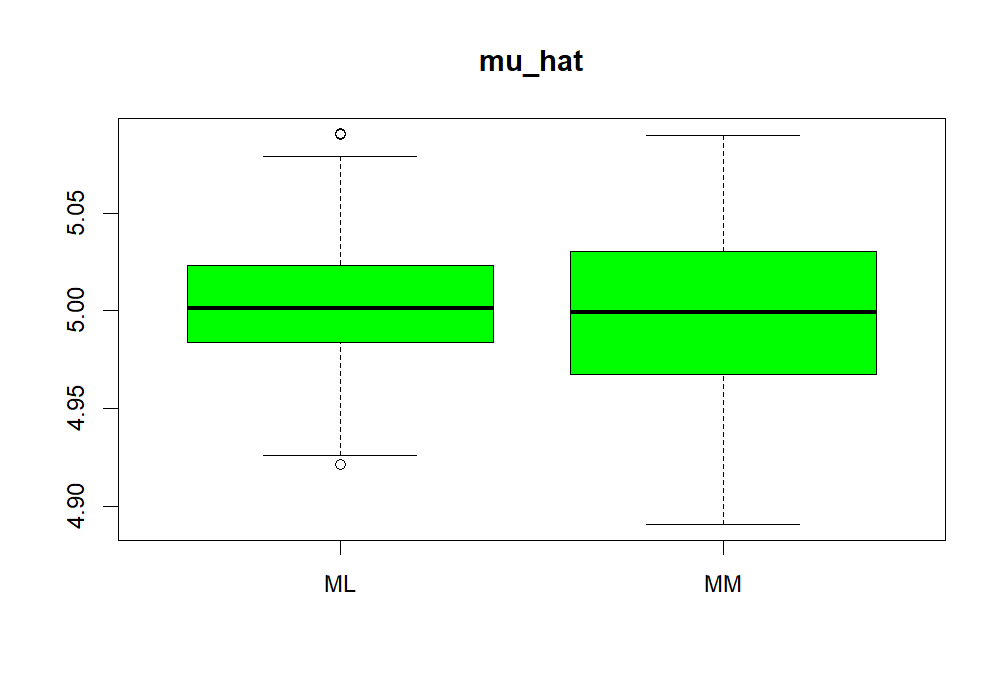
\includegraphics[scale=0.6]{task_1_mu.png}

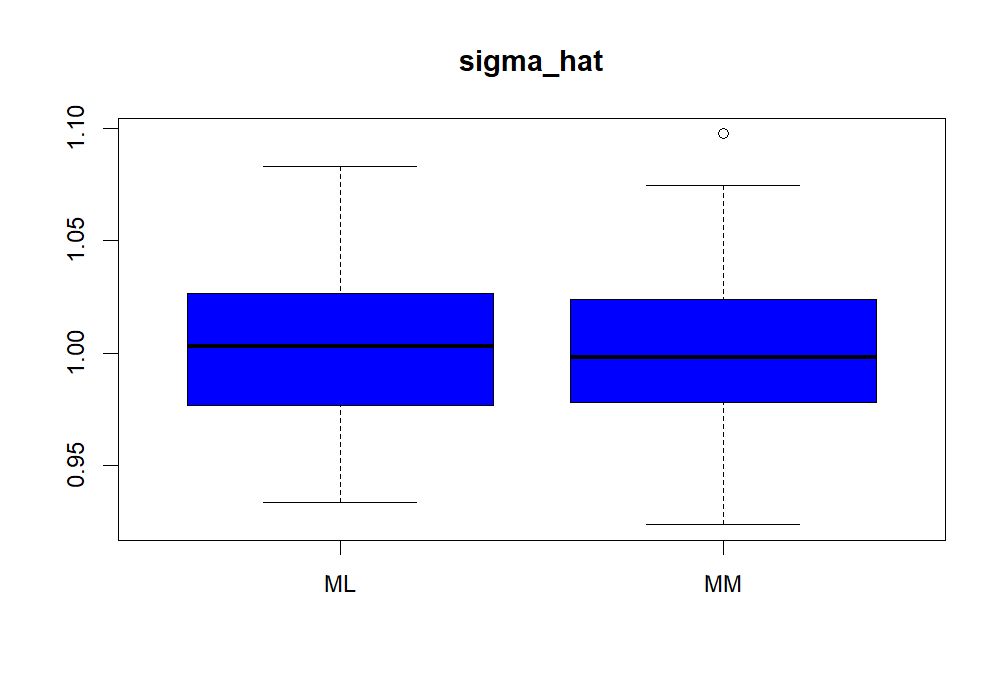
\includegraphics[scale=0.6]{task_1_sigma.png}
\end{problem}

\begin{problem}{5}
\begin{lstlisting}[language=R]
theta = 2

n = 1000
x = rexp(n, theta)

N = 100
LEFT = 2
RIGHT = 2.5
t = seq(LEFT, RIGHT, (RIGHT-LEFT)/(N-1))

f_hat = rep(NA, N)

for (i in 1:N) {
  if (sum(x) > t[i]) {
    f_hat[i] = (1 - t[i] / sum(x))^(n - 1)
  } else {
    f_hat[i] = 0
  }
}

plot(t, f_hat, type="l", main = "Graphs f", xlim = c(LEFT, RIGHT),
	col="black")

f = rep(NA, N)
f = exp(-theta*t)
lines(t, f, type="l",col="red")

f_hat_3 = rep(NA, N)
x_1 = rexp(n, theta)
x_2 = rexp(n, theta)
x_3 = rexp(n, theta)
for (i in 1:N) {
  if(sum(x)>t[i] && sum(x_2)>t[i] && sum(x_3)>t[i]) {
    f_hat_3[i] = ((1-t[i]/sum(x_1))^(n-1) + (1-t[i]/sum(x_2))^(n-1) 
	+ (1-t[i]/sum(x_3))^(n-1))/3
  } else {
    f_hat_3[i] = 0
  }
}

lines(t, f_hat_3,type="l",col="green")

legend(x = "topright", legend = c("f_hat", "f", "f_hat_3"),
col = c("black", "red", "green"), lwd = 2) 
\end{lstlisting}
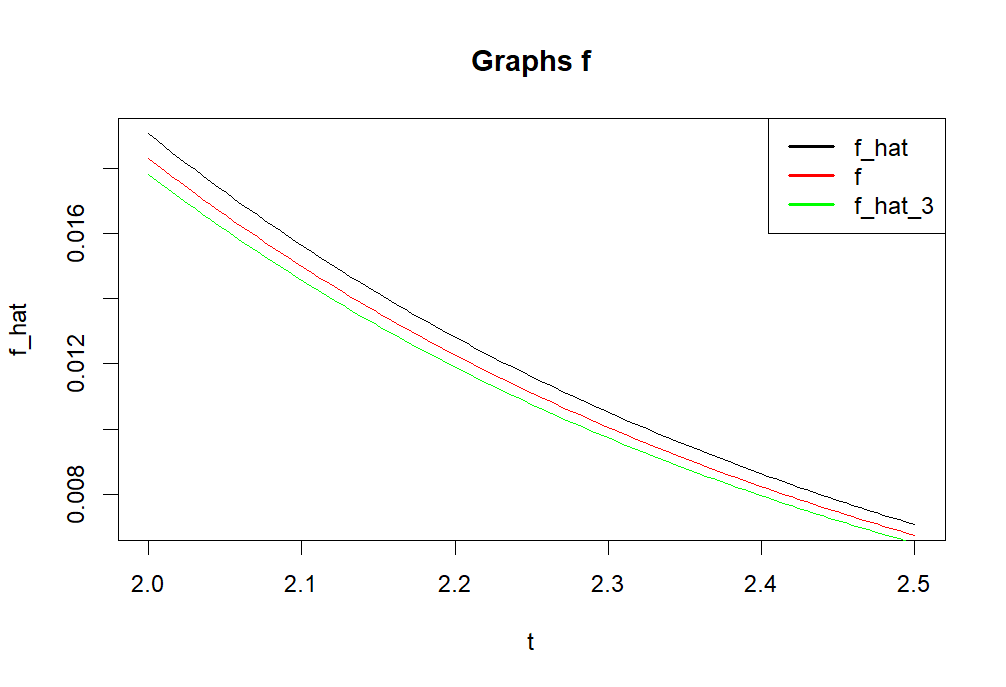
\includegraphics[scale=0.6]{task_2_f.png}
\end{problem}

\begin{problem}{5}
$$F(x_{1/2}) = \frac{1}{2} \ \ \ \ \ \ 1 - e^{-5x_{1/2}} = \frac{1}{2} \ \ \ \ \ \  x_{1/2} = \frac{\mathrm{log}2}{5}$$
$$\sigma^2 := \left( 2p\left(x_{1/2}\right)\right)^{-2} = \left( 2\theta e^{-\theta x_{1/2}}\right)^{-2} = 
\left( 2 \cdot 5 e^{-\mathrm{log}2}\right)^{-2} = 0.04
$$
\begin{lstlisting}[language=R]
theta = 5
x_m = log(2)/5
sigma_m = (10*exp(-5*x_m))^(-2)
M = 100

sigma1=rep(NA,M)
sigma2=rep(NA,M)
sigma3=rep(NA,M)

n = 1000
diff = rep(NA,M)
for (i in 1:M) {
  x = rexp(n, theta)
  diff[i] = sqrt(n)*(median(x)-x_m)
  sigma1[i] = sum((x - mean(x))^2)/(length(x) - 1)
}
qqnorm(diff, main="QQ-plot: n = 1000")
qqline(diff)

n = 10000
diff = rep(NA,M)

for (i in 1:M) {
  x = rexp(n, theta)
  diff[i] = sqrt(n)*(median(x)-x_m)
  sigma2[i] = sum((x - mean(x))^2)/(length(x) - 1)
}
qqnorm(diff, main="QQ-plot: n = 10000")
qqline(diff)

n = 100000
diff = rep(NA,M)
for (i in 1:M) {
  x = rexp(n, theta)
  diff[i] = sqrt(n)*(median(x)-x_m)
  sigma3[i] = sum((x - mean(x))^2)/(length(x) - 1)
}
qqnorm(diff, main="QQ-plot: n = 100000")
qqline(diff)


boxplot(sigma1, sigma2, sigma3, xaxt="n")
axis(side=1,at=1:3,label=c("1000","10000", "100000"))
\end{lstlisting}
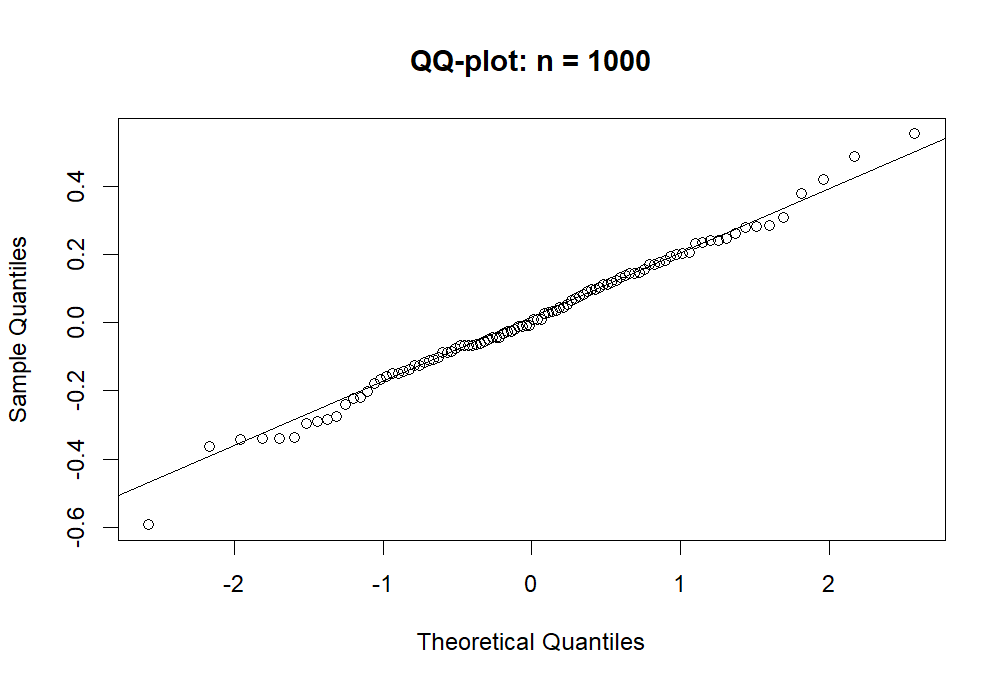
\includegraphics[scale=0.6]{task_3_qqp_n1000.png}

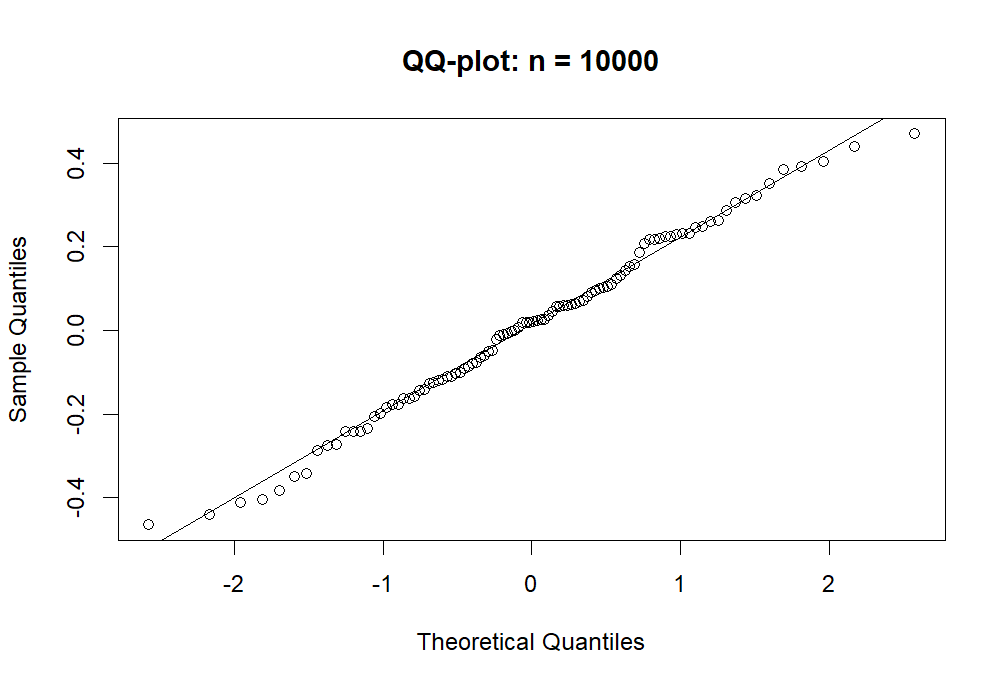
\includegraphics[scale=0.6]{task_3_qqp_n10000.png}

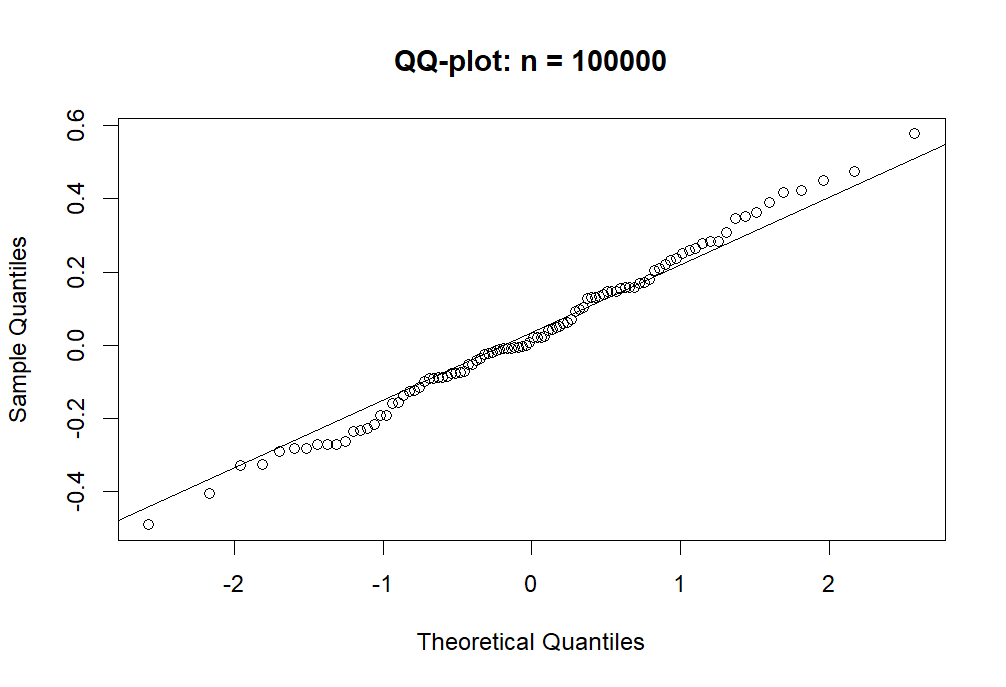
\includegraphics[scale=0.6]{task_3_qqp_n100000.png}

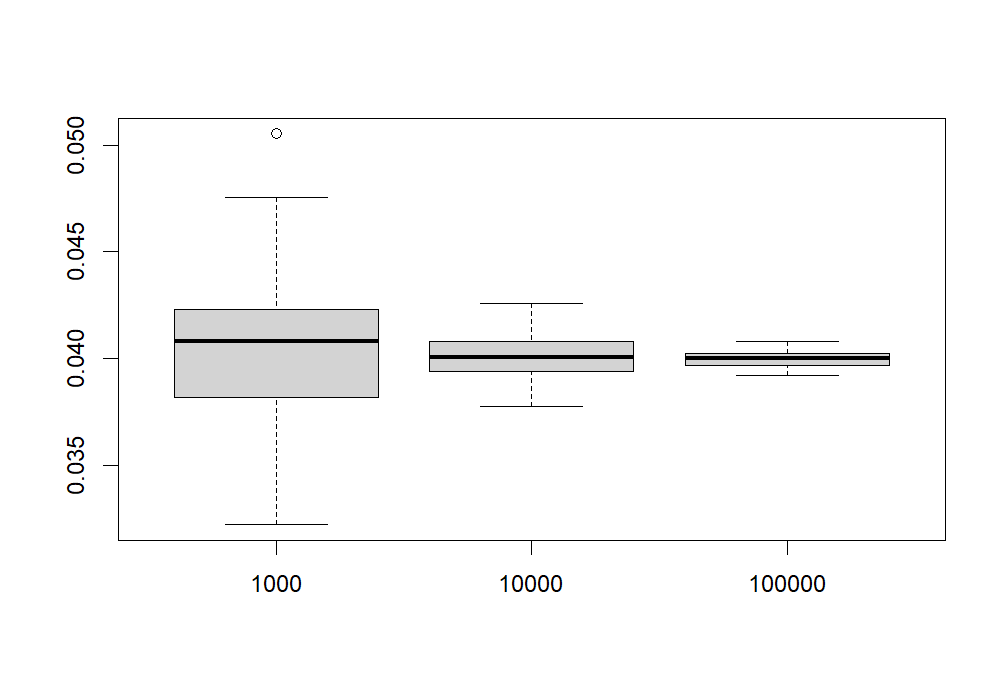
\includegraphics[scale=0.6]{task_3_sigma.png}

\end{problem}

\begin{problem}
\begin{lstlisting}[language=R]
x = ibm[1:369]
y = rep(NA,368)

for (i in 1:368) {
  y[i] = (log(x[i+1]/x[i])) * (log(x[i+1]/x[i])) 
}

plot(y)

theta = mean(y)

lambda = 1/mean(y)

yorder = sort(y)
x = rep(NA,368)
for (i in 1:368) {
  x[i] = i/368
}
plot(yorder, x,type="l")


F1 = rep(NA, N)
F1 = pnorm(sqrt(yorder), 0, theta) - pnorm(-sqrt(yorder), 0, theta)
lines(yorder, F1, type="l",col="red")

F2 = rep(NA, N)
F2 = 1 - exp(-lambda*yorder)
lines(yorder, F2, type="l",col="blue")
        
legend(x = "topright", legend = c("actual", "F1", "F2"), col = c("black", "red", "blue"), lwd = 2) 
\end{lstlisting}

Показательное распределение с неизвестным параметром лучше приближает данные      

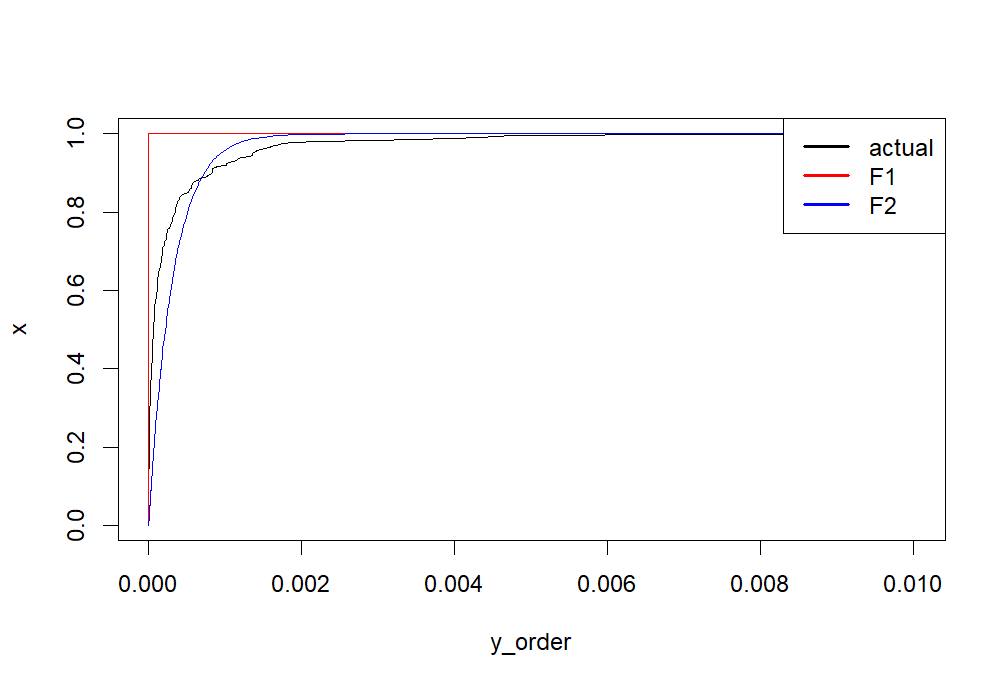
\includegraphics[scale=0.6]{task_4.png}

\end{problem}

\end{document}
  